\documentclass{standalone}
\usepackage{tikz}
\usetikzlibrary{patterns, positioning}
\usepackage[sfdefault]{ClearSans} %% option 'sfdefault' activates Clear Sans as the default text font
\usepackage[T1]{fontenc}

\begin{document}
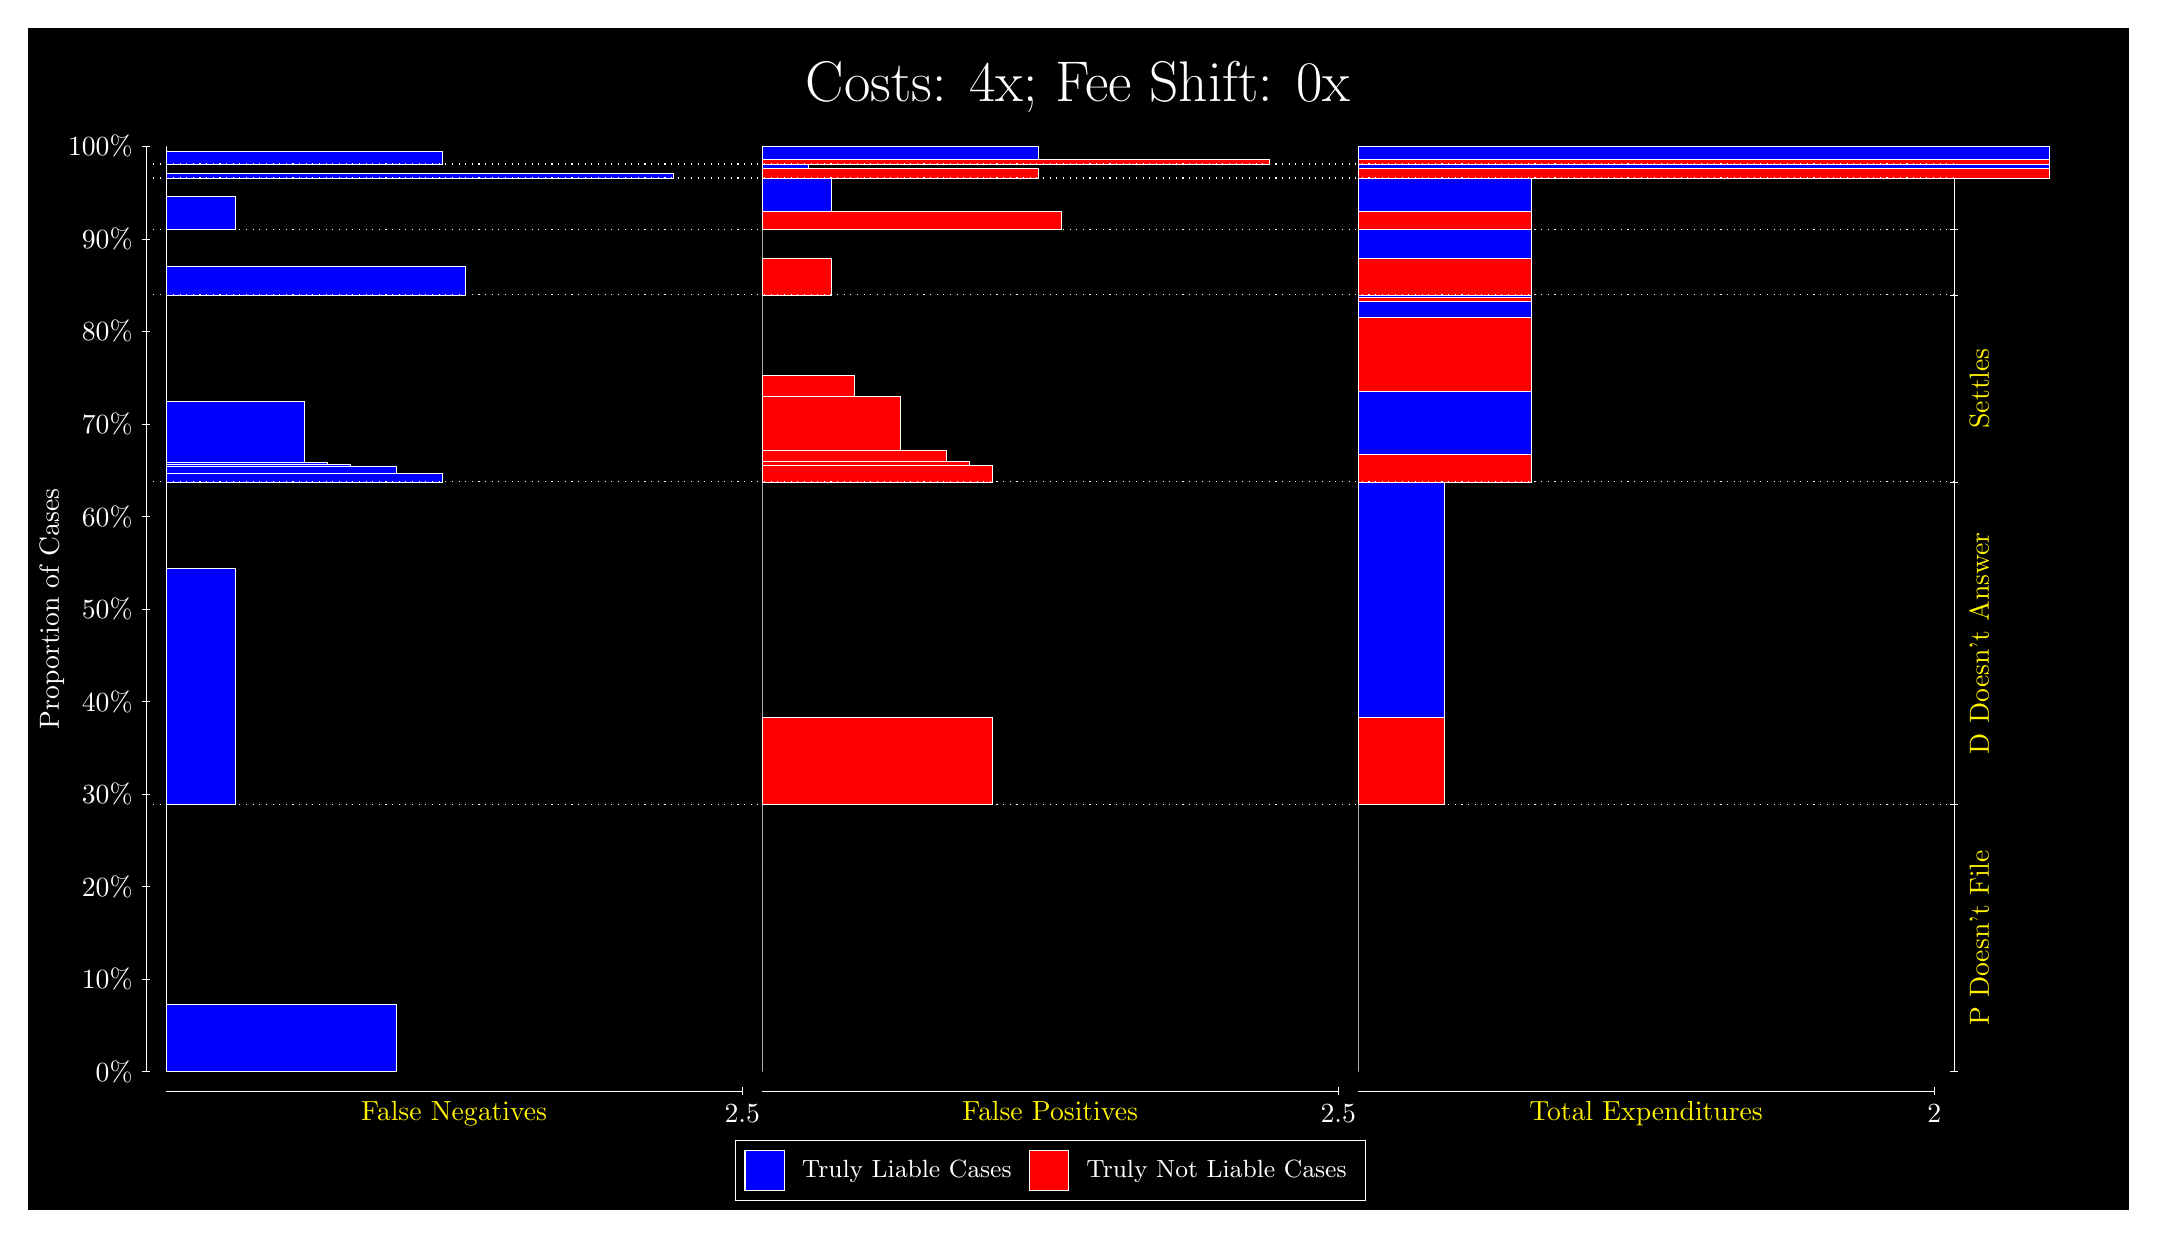
\begin{tikzpicture}
\draw[fill=black] (0,0) rectangle (26.667,15);
\draw[text=white] (0,13.5) rectangle (26.667,15) node[midway] {\huge Costs: 4x; Fee Shift: 0x};
\draw[white, very thin] (1.5,1.75) -- (1.5,13.5);
\node[rotate=90, text=white, anchor=center] at (0.3, 7.625) {Proportion of Cases};
\draw[white, very thin] (1.45,1.75) -- (1.55,1.75);
\node[text=white, anchor=east] at (1.45, 1.75) {0\%};
\draw[white, very thin] (1.45,2.925) -- (1.55,2.925);
\node[text=white, anchor=east] at (1.45, 2.925) {10\%};
\draw[white, very thin] (1.45,4.1) -- (1.55,4.1);
\node[text=white, anchor=east] at (1.45, 4.1) {20\%};
\draw[white, very thin] (1.45,5.275) -- (1.55,5.275);
\node[text=white, anchor=east] at (1.45, 5.275) {30\%};
\draw[white, very thin] (1.45,6.45) -- (1.55,6.45);
\node[text=white, anchor=east] at (1.45, 6.45) {40\%};
\draw[white, very thin] (1.45,7.625) -- (1.55,7.625);
\node[text=white, anchor=east] at (1.45, 7.625) {50\%};
\draw[white, very thin] (1.45,8.8) -- (1.55,8.8);
\node[text=white, anchor=east] at (1.45, 8.8) {60\%};
\draw[white, very thin] (1.45,9.975) -- (1.55,9.975);
\node[text=white, anchor=east] at (1.45, 9.975) {70\%};
\draw[white, very thin] (1.45,11.15) -- (1.55,11.15);
\node[text=white, anchor=east] at (1.45, 11.15) {80\%};
\draw[white, very thin] (1.45,12.325) -- (1.55,12.325);
\node[text=white, anchor=east] at (1.45, 12.325) {90\%};
\draw[white, very thin] (1.45,13.5) -- (1.55,13.5);
\node[text=white, anchor=east] at (1.45, 13.5) {100\%};

\draw[white, very thin] (24.457,1.75) -- (24.457,13.5);
\draw[white, very thin] (24.407,1.75) -- (24.507,1.75);
\node[anchor=west] at (24.407, 1.75) {};
\draw[white, very thin] (24.407,5.1418) -- (24.507,5.1418);
\node[anchor=west] at (24.407, 5.1418) {};
\draw[white, very thin] (24.407,9.2382) -- (24.507,9.2382);
\node[anchor=west] at (24.407, 9.2382) {};
\draw[white, very thin] (24.407,11.613) -- (24.507,11.613);
\node[anchor=west] at (24.407, 11.613) {};
\draw[white, very thin] (24.407,12.442) -- (24.507,12.442);
\node[anchor=west] at (24.407, 12.442) {};
\draw[white, very thin] (24.407,13.098) -- (24.507,13.098);
\node[anchor=west] at (24.407, 13.098) {};
\draw[white, very thin] (24.407,13.275) -- (24.507,13.275);
\node[anchor=west] at (24.407, 13.275) {};
\draw[white, very thin] (24.407,13.5) -- (24.507,13.5);
\node[anchor=west] at (24.407, 13.5) {};

\draw[white, very thin, fill=blue] (1.75,1.75) rectangle (4.6775,2.6019);
\draw[white, very thin, fill=red] (1.75,2.6019) rectangle (1.75,5.1418);
\draw[white, very thin, fill=blue] (1.75,5.1418) rectangle (2.6283,8.1355);
\draw[white, very thin, fill=red] (1.75,8.1355) rectangle (1.75,9.2382);
\draw[white, very thin, fill=blue] (1.75,9.2382) rectangle (5.2631,9.3481);
\draw[white, very thin, fill=blue] (1.75,9.3481) rectangle (4.6775,9.435);
\draw[white, very thin, fill=blue] (1.75,9.435) rectangle (4.092,9.4614);
\draw[white, very thin, fill=blue] (1.75,9.4614) rectangle (3.7993,9.4919);
\draw[white, very thin, fill=blue] (1.75,9.4919) rectangle (3.5065,10.26);
\draw[white, very thin, fill=red] (1.75,10.26) rectangle (1.75,11.613);
\draw[white, very thin, fill=blue] (1.75,11.613) rectangle (5.5558,11.978);
\draw[white, very thin, fill=red] (1.75,11.978) rectangle (1.75,12.442);
\draw[white, very thin, fill=blue] (1.75,12.442) rectangle (2.6283,12.86);
\draw[white, very thin, fill=red] (1.75,12.86) rectangle (1.75,13.098);
\draw[white, very thin, fill=blue] (1.75,13.098) rectangle (8.1906,13.158);
\draw[white, very thin, fill=red] (1.75,13.158) rectangle (1.75,13.275);
\draw[white, very thin, fill=blue] (1.75,13.275) rectangle (5.2631,13.44);
\draw[white, very thin, fill=red] (1.75,13.44) rectangle (1.75,13.5);
\draw[white, very thin, fill=red] (9.3189,1.75) rectangle (9.3189,4.2899);
\draw[white, very thin, fill=blue] (9.3189,4.2899) rectangle (9.3189,5.1418);
\draw[white, very thin, fill=red] (9.3189,5.1418) rectangle (12.246,6.2445);
\draw[white, very thin, fill=blue] (9.3189,6.2445) rectangle (9.3189,9.2382);
\draw[white, very thin, fill=red] (9.3189,9.2382) rectangle (12.246,9.449);
\draw[white, very thin, fill=red] (9.3189,9.449) rectangle (11.954,9.5039);
\draw[white, very thin, fill=red] (9.3189,9.5039) rectangle (11.661,9.6454);
\draw[white, very thin, fill=red] (9.3189,9.6454) rectangle (11.075,10.328);
\draw[white, very thin, fill=red] (9.3189,10.328) rectangle (10.49,10.591);
\draw[white, very thin, fill=blue] (9.3189,10.591) rectangle (9.3189,11.613);
\draw[white, very thin, fill=red] (9.3189,11.613) rectangle (10.197,12.077);
\draw[white, very thin, fill=blue] (9.3189,12.077) rectangle (9.3189,12.442);
\draw[white, very thin, fill=red] (9.3189,12.442) rectangle (13.125,12.68);
\draw[white, very thin, fill=blue] (9.3189,12.68) rectangle (10.197,13.098);
\draw[white, very thin, fill=red] (9.3189,13.098) rectangle (12.832,13.215);
\draw[white, very thin, fill=blue] (9.3189,13.215) rectangle (9.9044,13.275);
\draw[white, very thin, fill=red] (9.3189,13.275) rectangle (15.759,13.335);
\draw[white, very thin, fill=blue] (9.3189,13.335) rectangle (12.832,13.5);
\draw[white, very thin, fill=red] (16.888,1.75) rectangle (16.888,4.2899);
\draw[white, very thin, fill=blue] (16.888,4.2899) rectangle (16.888,5.1418);
\draw[white, very thin, fill=red] (16.888,5.1418) rectangle (17.986,6.2445);
\draw[white, very thin, fill=blue] (16.888,6.2445) rectangle (17.986,9.2382);
\draw[white, very thin, fill=red] (16.888,9.2382) rectangle (19.083,9.5905);
\draw[white, very thin, fill=blue] (16.888,9.5905) rectangle (19.083,10.385);
\draw[white, very thin, fill=red] (16.888,10.385) rectangle (19.083,11.331);
\draw[white, very thin, fill=blue] (16.888,11.331) rectangle (19.083,11.528);
\draw[white, very thin, fill=red] (16.888,11.528) rectangle (19.083,11.582);
\draw[white, very thin, fill=blue] (16.888,11.582) rectangle (19.083,11.613);
\draw[white, very thin, fill=red] (16.888,11.613) rectangle (19.083,12.077);
\draw[white, very thin, fill=blue] (16.888,12.077) rectangle (19.083,12.442);
\draw[white, very thin, fill=red] (16.888,12.442) rectangle (19.083,12.68);
\draw[white, very thin, fill=blue] (16.888,12.68) rectangle (19.083,13.098);
\draw[white, very thin, fill=red] (16.888,13.098) rectangle (25.67,13.215);
\draw[white, very thin, fill=blue] (16.888,13.215) rectangle (25.67,13.275);
\draw[white, very thin, fill=red] (16.888,13.275) rectangle (25.67,13.335);
\draw[white, very thin, fill=blue] (16.888,13.335) rectangle (25.67,13.5);
\draw[white, dotted] (1.5,5.1418) -- (24.457,5.1418);
\draw[white, dotted] (1.5,9.2382) -- (24.457,9.2382);
\draw[white, dotted] (1.5,11.613) -- (24.457,11.613);
\draw[white, dotted] (1.5,12.442) -- (24.457,12.442);
\draw[white, dotted] (1.5,13.098) -- (24.457,13.098);
\draw[white, dotted] (1.5,13.275) -- (24.457,13.275);
\draw[white, very thin] (1.75,1.5) -- (9.0689,1.5);
\node[text=yellow, anchor=north] at (5.4094, 1.5) {False Negatives};
\draw[white, very thin] (9.0689,1.45) -- (9.0689,1.55);
\node[text=white, anchor=north] at (9.0689, 1.45) {2.5};

\draw[white, very thin] (9.3189,1.5) -- (16.638,1.5);
\node[text=yellow, anchor=north] at (12.978, 1.5) {False Positives};
\draw[white, very thin] (16.638,1.45) -- (16.638,1.55);
\node[text=white, anchor=north] at (16.638, 1.45) {2.5};

\draw[white, very thin] (16.888,1.5) -- (24.207,1.5);
\node[text=yellow, anchor=north] at (20.547, 1.5) {Total Expenditures};
\draw[white, very thin] (24.207,1.45) -- (24.207,1.55);
\node[text=white, anchor=north] at (24.207, 1.45) {2};

\node[text=yellow, centered, rotate=90] at (24.777, 3.4459) {P Doesn't File};
\node[text=yellow, centered, rotate=90] at (24.777, 7.19) {D Doesn't Answer};
\node[text=yellow, centered, rotate=90] at (24.777, 10.426) {Settles};





\draw (12.978300999999998,1.5) node[draw=none] (baseCoordinate) {};
\begin{scope}[align=center]
        \matrix[scale=0.5, draw=white, below=0.5cm of baseCoordinate, nodes={draw}, column sep=0.1cm]{
            \node[rectangle, draw, minimum width=0.5cm, minimum height=0.5cm, fill=blue] {}; &
            \node[draw=none, font=\small, text=white] (B) {Truly Liable Cases}; &
            \node[rectangle, draw, minimum width=0.5cm, minimum height=0.5cm, fill=red] {}; &
            \node[draw=none, font=\small, text=white] (B) {Truly Not Liable Cases}; \\
            };
\end{scope}

\end{tikzpicture}
\end{document}